%%%%%%%%%%%%%%%%%%%%%%%%%%%%%%%%%%%%%%%%%%%%%%%%%%%%%%%%%%%%%%%%%%%%%%%%%%%%%%%
% Definici�n del tipo de documento.                                           %
% Posibles tipos de papel: a4paper, letterpaper, legalpapper                  %
% Posibles tama�os de letra: 10pt, 11pt, 12pt                                 %
% Posibles clases de documentos: article, report, book, slides                %
%%%%%%%%%%%%%%%%%%%%%%%%%%%%%%%%%%%%%%%%%%%%%%%%%%%%%%%%%%%%%%%%%%%%%%%%%%%%%%%
\documentclass[10pt, spanish, a4paper]{article}

%%%%%%%%%%%%%%%%%%%%%%%%%%%%%%%%%%%%%%%%%%%%%%%%%%%%%%%%%%%%%%%%%%%%%%%%%%%%%%%
% Los paquetes permiten ampliar las capacidades de LaTeX.                     %
%%%%%%%%%%%%%%%%%%%%%%%%%%%%%%%%%%%%%%%%%%%%%%%%%%%%%%%%%%%%%%%%%%%%%%%%%%%%%%%
\usepackage[spanish]{babel}     % Paquete para definir el idioma usado.
\usepackage[latin1]{inputenc}   % Define la codificaci�n de caracteres 
                                % (latin1 es ISO 8859-1)
%\usepackage[T1]{fontenc}        % Agrega caracteres extendidos al font
\usepackage{t1enc}
\usepackage{palatino}           % Cambia el font por omision a Palatino
\usepackage{graphicx}           % Paquete para inclusi�n de gr�ficos.
%%%%%%%%%%%%%%%%%%%%%%%%%%%%%%%%%%%%%%%%%%%%%%%%%%%%%%%%%%%%%%%%%%%%%%%%%%%%%%%

% T��tulo principal del documento.
\title{\textbf{The Speaker (2da Entrega)}}

% Informaci�n sobre los autores.
\author{    
            Juan Manuel Barrenche, \textit{Padr�n Nro. 86.152}                 \\
            \texttt{ snipperme@gmail.com }                                     \\
            Mart��n Fern�ndez, \textit{Padr�n Nro. 88.171}                      \\
            \texttt{ tinchof@gmail.com }                                       \\
            Marcos J. Medrano, \textit{Padr�n Nro. 86.729}                     \\
            \texttt{ marcosmedrano0@gmail.com }                                \\
            Federico Valido, \textit{Padr�n Nro. 82.490}                       \\
            \texttt{ fvalido@gmail.com }                                       \\ 
                                                                               \\
            \normalsize{Grupo Nro. 11 (YES)}                                   \\
            \normalsize{Ayudante: Renzo Navas}                         	       \\
            \normalsize{1er. Cuatrimestre de 2009}                             \\
            \normalsize{75.06 Organizaci�n de Datos - Titular: Arturo Servetto}\\
            \normalsize{Facultad de Ingenier�a, Universidad de Buenos Aires}   \\
       }
\date{Domingo 10 de Mayo de 2009}


% Comienzo del documento
\begin{document}

\maketitle                % Inserta el t�tulo.
\thispagestyle{empty}     % Quita el n�mero en la primer p�gina.

% Resumen que aparece en la primera p�gina (antes de la tabla de contenidos)
\begin{abstract}
El presente trabajo representa una aplicaci�n de los conceptos vistos durante
el m�dulo de \textit{Organizaci�n de Archivos} del curso de \textit{75.06 Organizaci�n de Datos} 
de la c�tedra Servetto.\\
\\
Consiste en implementar un sistema que permita la lectura de textos, la 
reproducci�n de los mismos en audio, y la indexaci�n de ellos. El usuario carga 
los audios correspondientes a cada termino encontrado en un archivo de texto, al
mismo tiempo que se indexan los t�rminos encontrados en el texto. El sistema debe ser capaz de 
persistirlos, recuperarlos y de reproducir de un texto, cada termino individual 
en base a las grabaciones cargadas previamente. \\
Este documento ha sido desarrollado en \LaTeX.
\end{abstract}

\newpage
\tableofcontents        % Comentar si no se desea la Table Of Content.
\newpage

% Inclusi�n de archivos externos
\section{Arquitectura}

El Main ser� simplemente una vista de WordService que es el backend de la aplicaci�n y quien brinda todos los servicios a la vista. Estos servicios son:
\begin{enumerate}
\item Agregar un Documento.
\item Realizar una b�squeda.
\item Reproducir un Documento.
\end{enumerate}

Veamos la arquitectura parte por parte. Pero antes definamos el concepto de Documento, que es com�n a todas las partes.

\subsection{Documento}

Es una interfaz que permite manejar un documento obteniendo de �l renglones.
Posee tres implementaciones, una que contiene un documento totalmente en memoria, otra que trabaja con un archivo que lee desde disco a medida que va necesit�ndolo, y otra que trabaja con los documentos prealmacenados que obtiene de forma \textit{lazy}.

Ahora si, veamos la arquitectura de cada una de las partes antes mencionadas.

\subsection{Agregar un Documento}

Se divide en divide en dos grandes partes:
\begin{enumerate}
\item Agregarlo al indice.
\item Agregarlo al diccionario de sonidos.
\end{enumerate}

Existe una caracter�stica en com�n entre estas dos partes: el parseo. Es por eso que la arquitectura se defini� de tal forma que el parseo se haga en una sola oportunidad como se mostrar� luego (esto tiene una peque�a consecuencia que se mencionar� al explicar la adici�n al diccionario de sonidos).

\subsubsection{Agregar un Documento al indice}


Quien se encarga de realizar esto es el \textit{Crawler}, quien recibir� un \textit{Documento}. En primer lugar le pasa el documento al \textit{Parser} que lo utilizar� como fuente para datos.

El Parser permite manejar un documento en forma de \textit{Frases}, entendiendo por tal a un conjunto de palabras separadas por un signo de puntuaci�n (\textit{'.', ',', ';', '?', '!'}, etc.). A estas frases les aplicar� un reemplazo de s�mbolos diacr�ticos, retiro de s�mbolos extra�os, s�mbolos num�ricos, etc, y case folding, obteniendo por resultado una lista de palabras limpia. De esta manera el \textit{Crawler} puede obtener \textit{Frases} limpias desde el parser al que inicialmente le pasa el documento como fuente.

La colecci�n de palabras obtenida ser� procesada por el m�dulo \textit{StopWords Discriminator}, cuya implementaci�n tendr� un listado en memoria (que levanta al iniciar la aplicaci�n desde un archivo) de frases y de palabras sueltas que son stop words para hacer el procesamiento.

El \textit{Crawler} obtiene del \textit{StopWords Discriminator} una colecci�n (ordenada o desordenada, no importa, pero con repeticiones, si importa) de palabras que no contienen stop words. Esta colecci�n (correspondiente a una sola \textit{Frase}) le ser� entregada al \textit{Indexer}.

El \textit{Indexer} es la interfaz utilizada para acceder al �ndice (un \textit{�rbol b\#}) (tambi�n podr�a haberselo llamado Index en vez de Indexer). El \textit{Crawler} maneja una session con el \textit{Indexer}, que comienza al procesar un \textit{Documento} y termina al agregar la �ltima \textit{Frase} (cuando el \textit{Parser} deja de brindarle datos). El \textit{Indexer} parametriza un \textit{BTree\#}, un m�dulo que maneja un �rbol b\# de manera gen�rica. El \textit{Indexer} a su vez maneja una session id�ntica a la que tiene con el \textit{Crawler} con el m�dulo \textit{Inversion Sort Handler}, y solo agregar� las palabras al �rbol una vez que el \textit{Crawler} finalice la session con el \textit{Indexer}.

El \textit{BTree\#} es una implementaci�n gen�rica de �rbol b\# que utiliza 2 archivos, uno para nodos internos y otro para hojas, y que maneja una equiparaci�n entre nodos y bloques. Utiliza el \textit{VariableLengthFileManager} en su implementaci�n en disco. Debe ser parametrizado con una \textit{Key} (clave de los nodos internos) y un \textit{Element} (registro de las hojas que contiene entre otras cosas a la clave). Este \textit{Element} se definir� de tal manera que tenga el listado de \textit{Documentos} en su interior; este listado de \textit{Documentos} se implementar� utilizado el \textit{VariableLengthFileManager}. No se muestra a \textit{Key} ni a \textit{Element}, ni al archivo del listado de \textit{Documentos} en el diagrama por simplificaci�n. Adem�s deben brindarse los \textit{Serializer} correspondientes a una colecci�n ordenada de \textit{Keys} y de \textit{Elements} para parametrizar al \textit{BTree\#}.

Las sessiones mencionadas (entre el \textit{Crawler} y \textit{Indexer}, y entre el \textit{Indexer} y el \textit{Inversion Sort Handler}) sirven para evitar tener un documento completo en memoria.

Al mismo tiempo que el \textit{Crawler} va procesando las frases, va a agregando todas las palabras encontradas en un Set (conjunto sin repeticiones), de esta manera obtiene el vocabulario completo. Ese Set ser� devuelto al \textit{WordService} como respuesta al pedido de indexar un documento.

\subsubsection{Agregar un Documento al diccionario de sonidos}

Como puede adivinarse, el vocabulario completo obtenido al agregar un docuemento al �ndice es la entrada usada para realizar el agregado al diccionario de sonidos. Esto tiene como consecuencia que el agregado de sonidos ser� en distinto orden al original del documento. Pero tiene como ventaja el no tener que procesar dos veces el documento por el \textit{Parser} (y a no tener que leerlo de nuevo desde disco si es que no se lo quiere tener completo en memoria como planteamos antes).

El m�dulo usado para esta acci�n es el llamado \textit{WordsRecorder}.

Si bien se modific� levemente la interacci�n entre los m�dulos, la arquitectura es b�sicamente la misma que para la entrega 1, y la interacci�n entre m�dulos puede verse claramente en el esquema.

La �nica gran modificaci�n consiste en el reemplazo del "�ndice secuencial de sonidos" por un \textit{Trie}, que utiliza para su implementaci�n un \textit{VariableLengthFileManager}.

\subsection{Realizar una B�squeda}

Esta acci�n es responsabilidad del \textit{Search Engine}. Para hacerlo primero debe limpiar la cadena de b�squeda, para lo cual interactura con el \textit{Parser} y con el \textit{StopWords Discriminator}.
Una vez que tiene la consulta limpia, realiza la b�squeda utilizando el \textit{Indexer}, que a su vez utilizar� el \textit{BTree\#}.

El \textit{SearchEngine} realiza las operaciones de ordenado necesarias y devuelve un listado ordenado de \textit{documentos}.

\subsection{Reproducir un Documento}

La reproducci�n la realizar� el \textit{DocumentPlayer}, que recibir� un \textit{Documento} que deber� parsear utilizando el \textit{Parser}. A medida que va obteniendo las palabras correspondientes las ir� reproduciendo delegando toda la complejidad en el \textit{WordsPlayer}.

El \textit{WordsPlayer} es la contrapartida del \textit{WordsRecorder} explicado antes, y su arquitectura es coincidente con la de este.

\subsection{VariableLengtFileManager - Archivo de registros de longitud variable en bloques}
El \textit{VariableLengthFileManager} que ya exist�a en la entrega anterior, ahora permite actualizaciones de los registros.
Recordemos que el \textit{Address} en este archivo consta de dos partes. La primera el bloque donde se encuentra el registro y la segunda el n�mero de objeto que representa el registro. Ahora bien, si una actualizaci�n de un registro aumentara el tama�o del mismo y esto hiciera que la suma de los tama�os de los registros que se encuentran en dicho bloque excediera el tama�o del bloque hay que hacer una reestructuraci�n de los datos. Existen varias alternativas para ello:
\begin{enumerate}
\item Tomar como pol�tica de reestructuraci�n la decisi�n de s�lo mover los objetos del final que excedan a la capacidad del bloque. Este es, para nuestro caso, impracticable ya que implicar�a actualizar todos los datos que tuvieran referencias a dichos objetos. 
\item Quitar �nicamente al objeto que se est� actualizando en dicho momento. Esto pareciera traer el mismo inconveniente, ya que al hacer esto, las direcciones de los subsiguientes registros tambi�n se ver�an modificadas porque en el bloque existe un objeto menos y el conteo quedar�a diferido en uno (es decir, que si quit� el registro cuyo n�mero de objeto 2 el siguiente, con n�mero de objeto 3, pasar�a a ser el objeto numero 2). 
\end{enumerate}
Entonces, para aplicar la segunda opci�n se debe evitar que los objetos siguientes al modificado mantengan su lugar en la lista. As� fue que se introdujo el concepto de \textbf{nullObject}.

\subsubsection{NullObject}
El \textbf{nullObject} es el encargado de ocupar el lugar que originalmente ocupaba un objeto que se encontraba compartiendo un bloque con otros registros y que, luego de su actualizaci�n, provoc� un desborde del bloque.
Ahora bien, recordemos que los objetos se encuentran serializados, y que la manera de rehidratandos es para todos la misma. Por lo cual necesitamos que los serializadores puedan hidratar \textbf{nullObject} sin intervenci�n de un proceso de verificaci�n, ni tener que estar agregando metadata listando los objetos que fueron retirados del bloque. Para ello se extendi� la interfaz \textit{Serializer} a una nueva llamada \textit{NullableSerializer} la cual indica que dicho serializador puede serializar e hidratar \textbf{nullObjects}. 
Todas nuestras implementaciones del NullObject se corresponden al valor \textbf{null} de Java, pero no tiene por qu� ser as�. El requisito es que el m�todo \textit{NullableSerializer\#dehydriateNull} modifique el Buffer de salida con, a lo sumo, el m�nimo tama�o de serializaci�n de los objetos no nulos y que adem�s, claro est�, el \textit{NullableSerializer\#hydrate} pueda interpretar esa informaci�n como un objeto mas (o la referencia \textbf{null}). Este requisito de m�ximo tama�o para la serializaci�n del \textbf{nullObject} se debe a que este objeto debe terminar ocupando menos que el objeto que lo que ocupaba el objeto a reemplazar antes de intentar ser modificado por el nuevo objeto. De esta manera, sabemos que, al quitarlo, los registros restantes y el \textbf{nullObject} van a caber en el bloque.

\subsubsection{Resultado final}
Finalmente las actualizaciones quedan de la siguiente manera y se distinguen tres casos de \textbf{desborde}:
\begin{enumerate}
\item Actualizaci�n de un registro que se encuentra solo en un bloque
\item Actualizaci�n de un registro que se encuentra como �ltimo registro del bloque
\item Actualizaci�n de un registro que no se encuentra como �ltimo registro del bloque
\end{enumerate}

\paragraph{Actualizaci�n de un registro que se encuentra solo en un bloque}

Este caso es el mas sencillo, ya que el registro est� solo y puede extenderse a m�ltiples bloques. Esto est� solucionado en los \textit{writers}, que agregar�n la metadata necesaria para asociar los bloques como si fueran uno solo. De manera que los \textit{readers} puedan leer toda la informaci�n en conjunto. \footnote{En este caso la direcci�n del objeto NUNCA cambia}

\paragraph{Actualizaci�n de un registro que se encuentra como �ltimo registro del bloque}

Este caso es el que le sigue en simplicidad. No requiere tampoco la intervenci�n de los \textbf{nullObjects}, solamente se retira el objeto del bloque y se lo hace ingresar nuevamente al archivo como una inserci�n. Esto nos devuelve una direcci�n que es la que se retorna como resultado de la actualizaci�n del registro para que el que solicit� la actualizaci�n modifique las referencias que pose�a hacia el registro.

\paragraph{Actualizaci�n de un registro que no se encuentra como �ltimo registro del bloque}

Al igual que en el caso anterior, se retira el objeto que se est� actualizando, pero esta vez se lo reemplaza por un \textbf{nullObject}. Nuevamente se procede al agregado del objeto al archivo por medio de una inserci�n que nos devolver� la nueva direcci�n del objeto que ser� enviada al que solicit� la actualizaci�n para que pueda actualizar todas las referencias que posee al objeto. Vemos que gracias a este concepto (\textbf{nullObject}) los casos quedaron todos similares y sin gran complejidad.

\paragraph{An�lisis de ventajas y desventajas}

Esta soluci�n permite que, a lo sumo, un �nico registro modifique su direcci�n y que dicho registro sea el que se solicit� actualizar, lo que nos garantiza que es un dato con el que se est� trabajando y que su \textit{Address} puede ser modificado donde sea pertinente. 

La desventaja que parece tener es que los bloques se empiezan a llenar con datos que no nos interesa almacenar (los \textbf{nullObjects}). Para evitar esto se pueden implementar pol�ticas de reorganizaci�n de bloques. �C�mo ser�a esto? Bueno, a simple vista se puede observar que si tengo que retirar el registro que se encuentra en la �ltima posicisi�n del bloque todos los nullObjects anteriores (hasta encontrar un objeto que no lo sea) pueden ser tambi�n retirados del bloque, ganando, de esta manera, mas espacio para los otros registros que se encuentran en el bloque y que ser� utilizado cuando dichos registros necesiten expandirse. Finalmente, cuando se actualice el �ltimo de los registros reales restantes en el bloque (es decir, el registro que se encuentra en un bloque donde, excluy�ndolo a �l mismo, en el bloque solo hay \textbf{nullObjects}) este puede retirar todas esas referencias a nullObjects quedando como �nico propietario del bloque. \footnote{Si bien estas pol�ticas no se encuentran implementadas, debido a falta de tiempo, son facilmente implementables y otorgan un mayor aprovechamiento del espacio reduciendo la fragmentaci�n interna}

\subsection{StraightVariableLengthFile - Archivo de registros de longitud variable sin bloques}

Se agreg� una forma mas de persistencia en archivos \textit{StraightVariableLengthFile}. Esta implementaci�n de archivo basa su funcionamiento en los mismos lineamientos que el \textit{VariableLengthFileManager} en la primera parte, exceptuando que no trabaja por bloques. Por lo cual cada registro es serializado a continuaci�n del �ltimo. Para recuperar un registro ya almacenado se recibe el \textit{Address} (que en este caso corresponde �nicamente a un Offset y que fue entregado por el \textit{StraightVariableLengthFile} al momento de agregarse dicho registro) y se utiliza el Serializador con que fue configurado para hidratar el registro que luego es devuelto al usuario. Las ventajas de esta implementaci�n, respecto a la de por bloques, es que los archivos quedan mas densos y no requiere meta data dentro del archivo (mas all� de la que requiera la serializaci�n, la cual es independiente de la implementaci�n del archivo).

Qued� pendiente, como idea, permitirle al usuario de ambos tipos de archivos (con y sin bloques) que posea una secci�n con datos reservados (al estilo meta-data) que puedan serializarse de manera diferente que el com�n de los registros. Observamos que esto ser�a �til en numerosos casos. Como simples ejemplos, si quisiera almacenar la cantidad de registros en el l�xico, si quisiera guardar en �rbol el nombre para el archivo de hojas, etc. Si bien, nuestros casos los resolvimos implementando serializadores con estado a los que se le indicaba que tipo de dato esperaban recibir, entendemos que esta configuraci�n complica algo que en concepto es mas sencillo.

\subsection{Otros datos relevantes de la arquitectura}

Se incorpor� la abstracci�n \textit{StraightVariableLengthFile} para el archivo de sonidos (que antes era un \textit{VariableLengthFileManager}) por lo que ahora el archivo correspondiente es 100\% denso. 

El \textit{VariableLengthFileManager} posee dos implementaciones, una que maneja cach� de bloques y la otra que no. La primera se usa en casos como el trie ya que todos los registros poseen un mismo serializador (recordemos que el trie est� implementado en dos archivos) y la segunda es utilizada en el �rbol, ya que la forma de los registros almacenados en los archivos var�a durante la vida del �rbol y esto fuerza al uso de un serializador mas dependiente del �rbol y esto complica el manejo del cach�.

\begin{figure}[!htp]
\centering
\makebox[\textwidth]{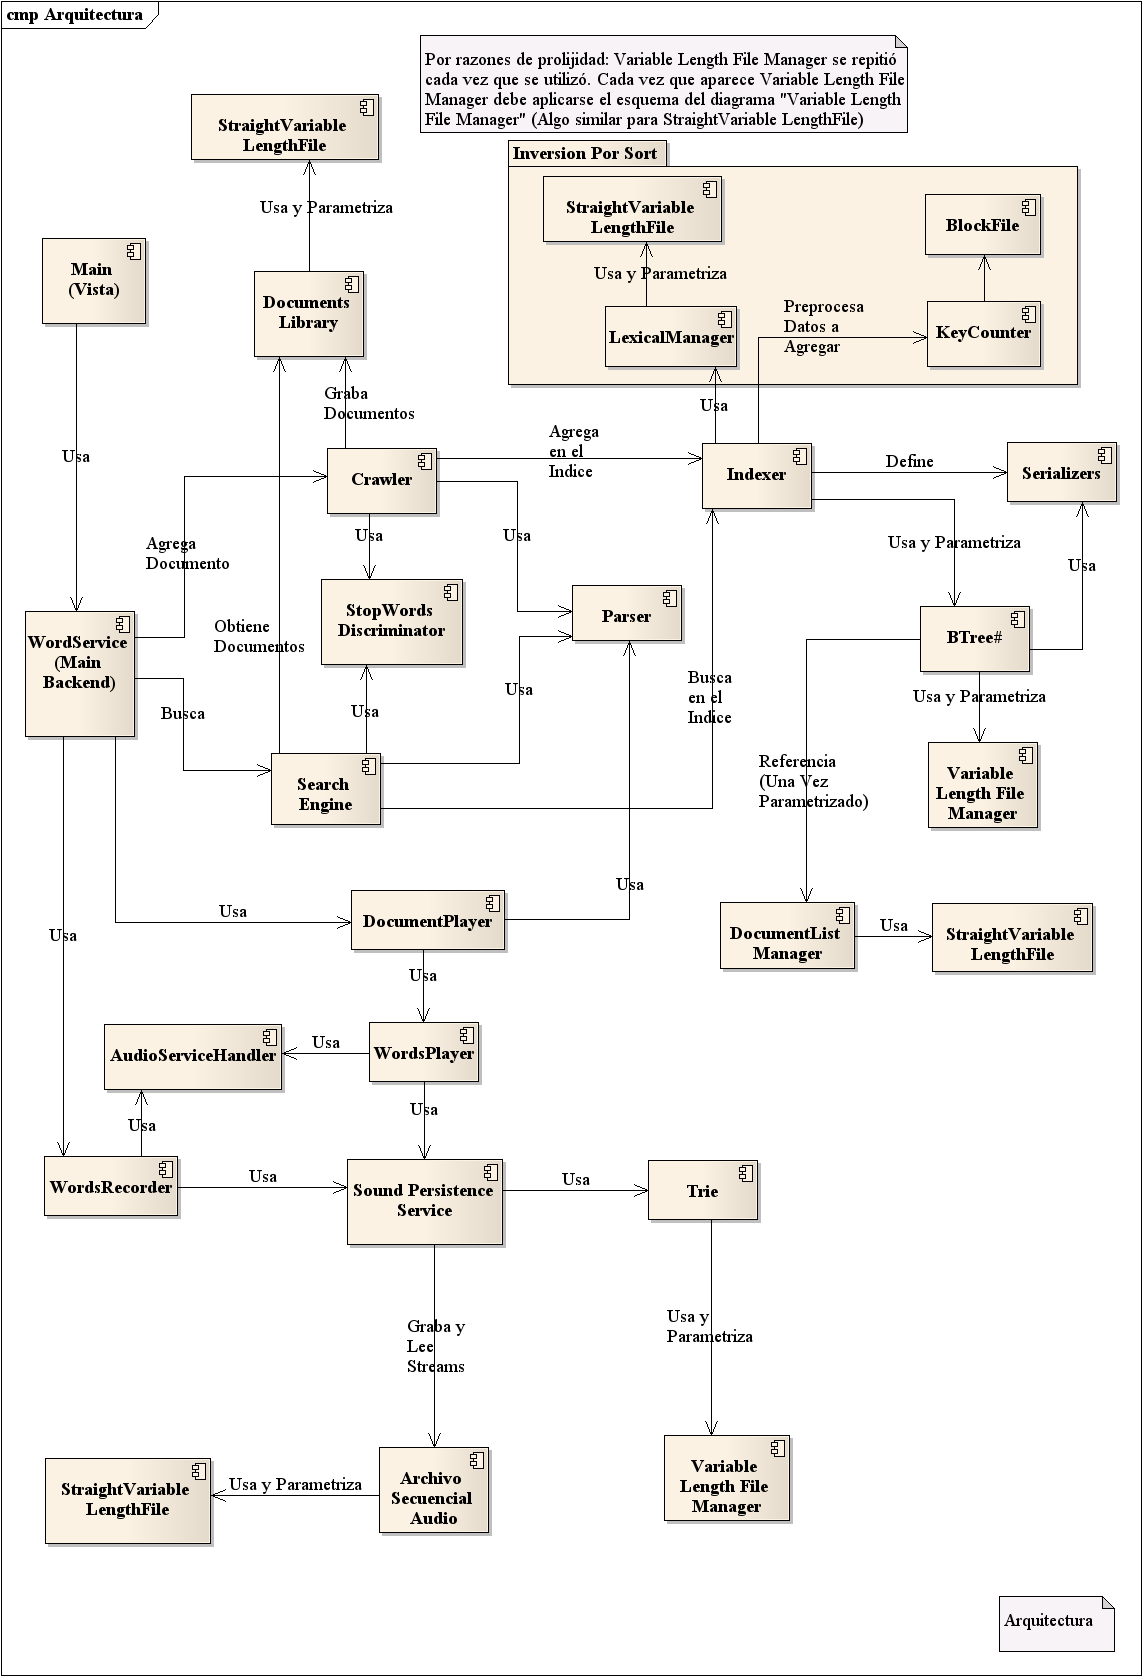
\includegraphics[scale=0.4,natwidth=20pt,natheight=10pt]{img/Arch2daEntrega.png}}
\caption{Arquitectura VariableLengthFileManager} 
\end{figure}

\begin{figure}[!htp]
\centering
\makebox[\textwidth]{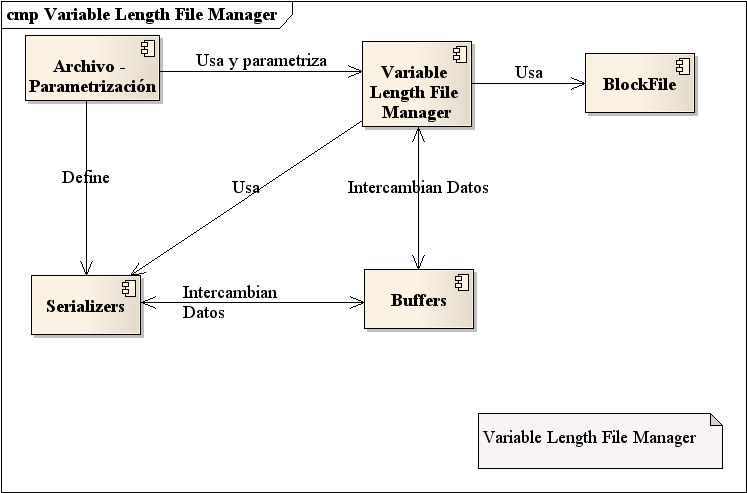
\includegraphics[scale=0.5,natwidth=20pt,natheight=10pt]{img/VariableLengthFileManager.png}}
\caption{Arquitectura VariableLengthFileManager}
\end{figure}

\begin{figure}[!htp]
\centering
\makebox[\textwidth]{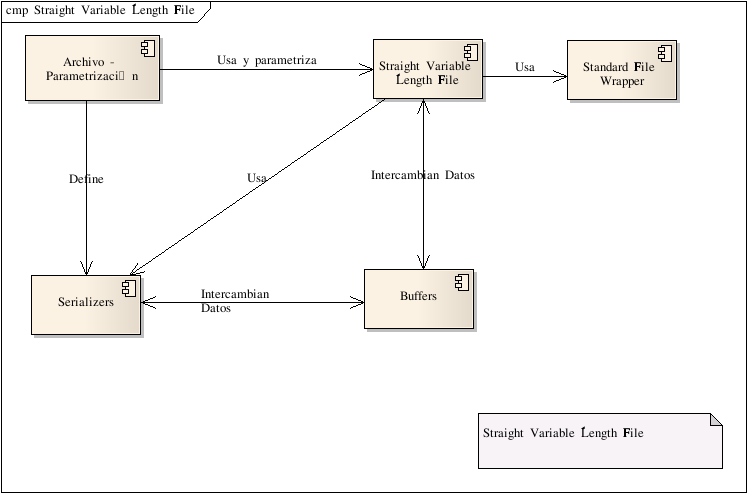
\includegraphics[scale=0.5,natwidth=20pt,natheight=10pt]{img/StraightVariableLengthFile.png}}
\caption{Arquitectura StraightVariableLengthFile}
\end{figure}


\section{Document Library}

\subsection{bla}
 % Document, DocumentLibrary
\section{Servicios de Documento (Backend)}
Dentro de este paquete se encuentra la clase principal de interaccion con el sistema, basicamente es lo unico que una 
View conoceria.

La clase \texttt{WordService} es el backend principal y punto de entrada a todo el sistema. Los servicios que expone 
son los que se detallaron en la secci�n de Arquitectura:
\begin{itemize}
  \item Agregar un documento
  \item Realizar una consulta
  \item Reproducir un documento
\end{itemize}

\subsection{WordService}

\paragraph{Interacciones}
Se encarga de instanciar el Indexador, el Crawler, el servicio de persistencia de sonidos (utilizando un Trie), la
librer�a de documentos y el SearchEngine, y orquestar las relaciones entre ellos.

\paragraph{Metodos}
Expone los metodos principales para agregar, buscar y reproducir documentos. Que son delegados a los demas objetos.

\paragraph{Conexion con View}
La conexion con View se hace explicitamente en los metodos par agregar y reproducir a traves de una interfase (IWordsRecordConnector), de esta manera el servicio no conoce especificamente que view lo utiliza.

\subsection{Crawler}
El crawler es una entidad bastante simple que se encarga de agregar documentos al sistema.

\paragraph{Agregar un documento al sistema}
El proceso de agregar un documento, consta de los siguientes pasos:

\begin{enumerate}
\item Agregar el documento a la Librer�a de Documentos.
\item Iniciar una sesi�n con el Indexador.
\item Pasar el documento al Parser que ira retornando las distintas frases.
\item Cada frase se pasa por el discriminador de stop words que devuelve solo los terminos relevantes.
\item Se indexan los terminos relevantes en el Indexador.
\item Una vez terminadas las frases del documentos, se cierra la sesi�n con el indexador.
\item Se devuelve el lexico completo del documento (incluyendo las stopwords).
\end{enumerate}

A continuaci�n se muestra un diagrama de secuencia de este proceso.

\begin{figure}[!htp]
\centering
\makebox[\textwidth]{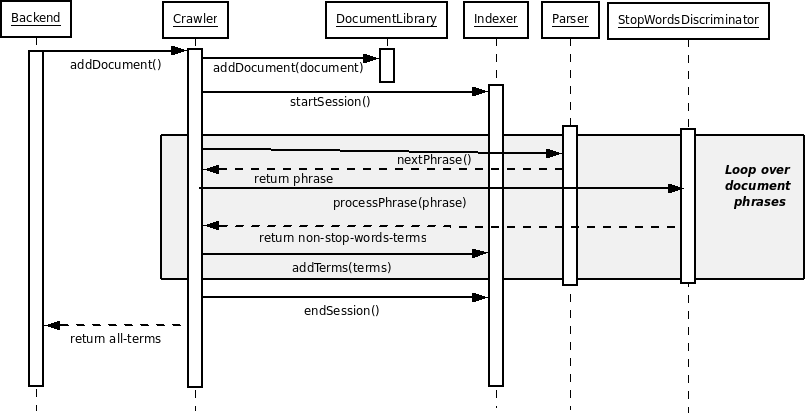
\includegraphics[scale=0.5,natwidth=20pt,natheight=10pt]{img/crawler.png}}
\caption{Diagrama de secuencia: Proceso de agregar un documento al sistema.} 
\end{figure}
     % Backend
\section{Filtros y Normalizaci�n de Documentos}

\subsection{Parser}
El Parser se encarga a partir de un Document de separarlo en frases u oraciones, siendo iterable por este criterio, es decir, por cada frase (identificada por un distintos separadores: "." , "!", "?", etc.) se tendra disponible una List<String> con cada palabra de la misma. Es importance mencionar que este modulo es lo sufientemente inteligente como para bufferizar las lineas del documento hasta encontrar una frase. 

\paragraph{Ejemplo}

\begin{verbatim}
1 - Primera Frase del documento. Segunda
2 - frase del documento. Tercera frase.
3 - Cuarta frase. Esta es la quinta
4 - frase del documento y continua por
5 - por mas de dos lineas.
\end{verbatim}

El parser devolvera estas 5 frases, siendo transparente para el que lo utilize en que linea empieza y termina cada una.

Ademas de separar las frases como explicamos anteriormente, se encarga de hacer CaseFolding y reemplazar o eliminar todos los caracteres diacriticos.


\subsection{StopWordsDiscriminator}

bla
\paragraph{stop}

bla
 % Crawler, Parser, Discriminator
%\section{Indexer}
\paragraph{Definici�n de Entidades}

Esta entidad es la encargada de manejar la generaci�n del indice invertido de documentos y t�rminos. Para ello se vale de tres herramientas principales: 
\begin{verbatim}
T�rminos indexados (Almacenados en el �rbol B#):
  Corresponde a cada t�rmino que se agrega al indexer. 
  Tiene asociada una lista de documentos que almacena 
  por fuera del �rbol B#. Dicha lista de documentos se
  almacena en un archivo por bloques con registros de 
  longitud variable.

Proceso de inversi�n por sort:
  Se sincroniza una nueva sesi�n por cada sesi�n que 
  se inicie en el indexer. Para que, cuando se le in-
  dique al Indexer que se finaliz� el agregado de in-
  formaci�n este pueda recuperar toda la informaci�n 
  ya ordenada y contada

Lexical Manager (Archivo de l�xico)
  Este es un simple archivo que contiene el l�xico 
  indexado.
\end{verbatim}
\subsection{Terminos indexados}
Los t�rminos indexados se encuentran representados por la clase \textbf{IndexerTreeElement} que implementa \textbf{Element} para poder almacenarse
como elemento del �rbol. Esta clase es parametrizable de manera que uno determina que es lo que quiere asociar a cada t�rmino (as� uno no tiene que restringirse a asociar, como en nuestro caso \textit{direcciones de la DocumentLibrary} y puede indicar de otra manera a que documento pertenece o bien indexar datos que no representen un documento.
Cada t�rmino indexado posee una lista de datos (cuyo tipo depende de como se parametriz� el Indexer) junto con la cantidad de veces que ocurri� el t�rmino para dicho dato. Esta lista se encuentra almacenada en un archivo externo al elemento, y es un archivo com�n para todos los elementos de un mismo indexer. La lista se almacena siempre ordenado decreciente respecto a la cantidad de ocurrencias.
El agregado de informaci�n a la lista se hace una �nica vez por \textit{"sesi�n del indexado"}, en el momento que se finaliza dicha sesi�n. Ah� se agregan los nuevos datos a la lista ya existente y se actualiza la lista en el archivo de listas \footnote{si bien, en la implementaci�n actual, nunca se agrega mas de un dato a la vez, ya que la interfaz agrega un �nico documento por vez, el circuito soporta que, durante una sesi�n, se indexen varios documentos}

\subsection{Inversi�n por sort}
El proceso de inversi�n por sort comienza cuando se inicia la sesi�n con el indexer. Este prepara un archivo de trabajo en el cual, mientras la sesi�n dure, se ir�n agregando elementos (en nuestro caso los elementos son la relaci�n \textit{id\_termino - id\_documento}). 
Cuando se da por finalizada la sesi�n, este proceso toma el archivo de trabajo de a partes (parametrizable por cantidad de registros) y realiza un sort externo. Es decir, cada parte es ordenada por separado en memoria y luego almacenada en otro archivo de trabajo. Luego a estos nuevos archivos se les realiza un merge (aprovechando el orden parcial que poseen) y para los casos que un mismo elemento se repite se aumenta la cantidad de ocurrencias del mismo y se almacena �nicamente una (con el total de ocurrencias) en un archivo resultado.
Este proceso, otorga al usuario, un iterador, para recorrer los elementos contados. Cuando el indexer itera sobre este resultado realiza un corte de control por \textit{id\_termino} para realizar una �nica actualizaci�n de la listas de dicho t�rmino.

\subsection{Lexical Manager}
El lexical m�nager es un archivo con registros de longitud variable que nos permite hacer la conversi�n entre un \textit{id\_termino} y t�rmino. Cada t�rmino almacenado en el �rbol B\# sharp posee adem�s su correspondiente \textit{id\_termino} que no var�a nunca. De manera que durante la sesi�n de indexado, por cada t�rmino a indexar se consulta el �ndice y se recupera este \textit{id\_termino} que es enviado, junto con el \textit{id\_documento}, al proceso de inversi�n por sort. Si no existiera el t�rmino en el �ndice, este es primero agregado al \textbf{Lexical Manager}, luego agregado al �ndice y finalmente enviado al proceso de inversi�n por sort.

\subsection{B�squedas}
Las consultas en el Indexer son siempre por t�rmino. Lo que resulta en una consulta que resuelve el �ndice, es decir, el �rbol B\#. El elemento recuperado es devuelto como un \textbf{IndexedTerm<T>} que le permite al que realiz� toda la consulta recuperar, de manera \textit{lazy}, los datos asociados al mismo y la cantidad de veces que ocurri� el t�rmino para cada dato. 

        % Indexer, LexicalManager ===> DESCOMENTAR CUANDO ESTE LA DOC DE JUAN !
\section{B# Tree}

\subsection{bla}
      % B# Tree
\section{SearchEngine: Queries y FTRS}

\subsection{bla}
    % SearchEngine, Queries, FTRS, etc.
\section{Diccionario de Palabras: Trie}
Para esta entrega, las palabras del diccionario fueron almacenadas en un Trie de profundidad parametrizable (por defecto 4). 
Esta estructura presenta una cualidad importante en nuestro contexto que es la optimizaci�n de las busquedas de claves. 
La b�squeda de una clave de longitud $n$ tendr� en el peor de los casos un orden de $O(m)$.

No se explicar�n aqu� todos los detalles espec�ficos de la estructura del Trie, sino que se har� referencia a alguno de
los detalles conceptualmente m�s importantes de la implementaci�n para este trabajo. \footnote{Puede encontrarse m�s
informaci�n en http://es.wikipedia.org/wiki/Trie}

\subsection{Implementaci�n en Disco}
A pesar de la estructura relativamente simple del Trie, este ocupa un tama�o considerable cuando se trata de almacenarlo
en disco por completo. La estructura en s� no impone ninguna limitaci�n sobre la cantidad de niveles que deba tener el
Trie, y este es un factor importante a tener en cuenta cuando la implementaci�n se hace en disco.

\paragraph{Profundidad del Trie}
Limitar la profundidad de niveles reduce el espacio necesario para almacenar el Trie, y generalmente es un requisito
de la implementaci�n en disco. Como consecuencia de la limitaci�n de niveles, el Trie pierde (en parte) su gran ventaja
que es la rapidez de las busquedas de claves. Esto puede verse claramente pensando que, al buscar una clave de longitud
mayor a N (siendo N la cantidad de niveles), solo se podr� bajar hasta el �ltimo nivel y luego se deber� hacer una 
busqueda secuencial (o binaria si se mantienen ordenadas) sobre el resto de las claves que compartan los mismas N primeros caracteres.

Considerando este problema, debemos encontrar una soluci�n de compromiso entre el espacio necesario para almacenar el
Trie y la rapidez de la busqueda de clavez que proporcionar�. Usualmente, limitando la cantidad de niveles a un valor 
entre 4 y 6, se logra una soluci�n bastante equilibrada.

\paragraph{Nodos Hojas: Cantidad de registros}
Otro problema que surge de la limitaci�n de la cantidad de niveles del Trie es la cantidad de registros que se necesitan
almacenar en los nodos hojas.

Debido a que muchas claves pueden tener en comun los primero caracteres, algunos nodos hojas pueden tener una cantidad
elevada de registros con terminaciones de claves, lo cual limita la posibilidad de levantar el nodo completo en memoria.
Para este problema se dise�o una soluci�n que explicaremos m�s adelante.

\subsection{Dise�o del Trie gen�rico}
Se intent� realizar una implementaci�n gen�rica del Trie. Para logra este objetivo, fue necesario definir interfaces 
extras que permitan trabajar con distintos tipos de datos.

\paragraph{Definici�n de Entidades}

Las entidades b�sicas son Element, Key y KeyAtom:

\begin{verbatim}
Elemento (Element):
  Es el elemento (o dato) que almacena el Trie.

Clave (Key):
  Es la clave mediante la cual se recorre el Trie. No necesariamente 
  debe ser una cadena de caract�res.

Porci�n de Clave (KeyAtom):
  Cada clave se divide en porciones ordenadas que se almacenan en 
  cada nivel. No necesariamente tiene que ser un caracter ya que 
  la clave podr�a dividirse en m�s de un caracteres. 
\end{verbatim}

Luego las entidades que le dan al Trie su estructura, InternalNode, LeafNode y NodeReference:

\begin{verbatim}
Referencia a Nodo (NodeReference): 
  Representa una referencia a un nodo (nodo hijo). Contiene 
  la direcci�n del nodo y la porci�n de clave del nodo hijo.
  
Nodo Interno (InternalNode):      
  Representa un nodo que no es hoja. Puede tener un dato si se
  agrega una clave que sea mas corta que la cantidad de niveles.
  
Nodo Hoja (LeafNode):
  Este nodo puede contener varios elementos ya que puede haber
  varios elementos cuya clave tengan el mismo comienzo. 
\end{verbatim}

\paragraph{Nodos}
Si no fuera por la limitaci�n de niveles, muy probablemente no ser�a necesario hacer una diferenciaci�n entre nodo
interno y nodo hoja. Sin embargo, en nuestro caso, los nodos hojas \textbf{nunca} contienen referencia a nodos hijos. 

\begin{figure}[!htp]
	\begin{center}
		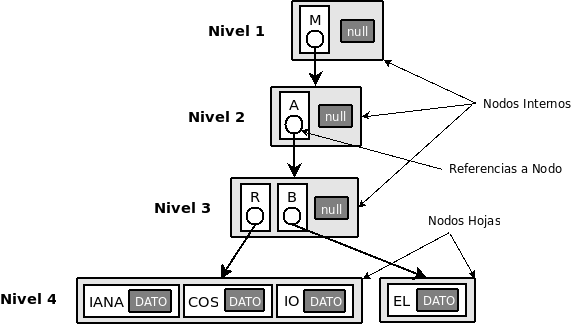
\includegraphics[scale=0.5,natwidth=20pt,natheight=10pt]{img/trie_simple.png}
	\end{center}
	\caption{Relaciones entre Nodos (Ej: Mariana,Marcos,Mario,Mabel)}
\end{figure}

\newpage

De la figura se puede prever que un nodo hoja podr�a eventualmente tener muchas terminaciones de claves (Mariana, Marcos
arcelo, Martes, Marciano, Mariano, Mario, etc). Si suponemos un numero considerable como 50 o 100 elementos en un nodo 
hoja, ya no podemos considerar que el nodo este por completo en memoria. 

Para solucionar este problema, se decidi� tratar a los nodos hojas con \textbf{particiones}. En vez de tener una entidad que 
represente un nodo hoja, se tiene una entidad que representa una parte de ese nodo hoja. De esta manera podemos levantar
a memoria, partes del nodo hoja y no el nodo completo.

Definimos entonces el concepto de \textbf{Partici�n de Nodo Hoja} \textbf{(LeafPartitionNode)}, el cual puede contener 
adentro una cantidad fija de registros. \footnote{Actualmente utilizamos una cantidad de 10 registros por partici�n.}

\begin{figure}[!htp]
	\begin{center}
		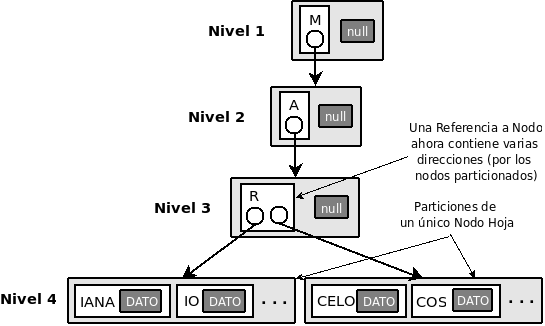
\includegraphics[scale=0.5,natwidth=20pt,natheight=10pt]{img/trie_particion.png}
	\end{center}
	\caption{Relaciones entre Nodos Internos y Nodos Hojas} 
\end{figure}

\subsection{Dise�o de Datos}
Teniendo en claro las entidades involucradas en la estructura del Trie, se realiz� un dise�o de los datos que ser�an
necesarios almacenar.

\begin{verbatim}
Nodo Interno: nivel, elemento (o dato), lista de referencias
Referencia a Nodo: porci�n de clave, lista de direcciones
Particion de Nodo Hoja: resto de la clave, elemento (o dato)
\end{verbatim}

Se implementaron dos archivos, ambos con \textbf{registros de longitud variable en bloques}, uno para los nodos registros
de los nodos internos y otro para los de nodos hojas.
\newpage
\paragraph{Dise�o Conceptual de Datos}
El dise�o conceptual de datos para los registros, queda:
\begin{verbatim}
Arhivo de nodos internos:
NodoInterno((nivel)1, (dato)?, referencia a nodo(porcion clave,
direccion((nro bloque)1, (nro objeto)1)*1 )*)

Archivo de nodos hojas:
ParticionNodoHoja( (resto clave((porcion clave)*))1, (dato)1 )
\end{verbatim}

\paragraph{Dise�o L�gico de Datos}
El dise�o l�gico de datos para los registros, queda:
\begin{verbatim}
Arhivo de nodos internos:
NodoInterno(nivel:Short, dato:Elemento, (porcion clave:KeyAtom, 
direccion(nro bloque:Long, nro objeto:Short)))

Archivo de nodos hojas:
ParticionNodoHoja(Cant de KeyAtom en resto de clave:Short, (porcion clave:KeyAtom), dato:Long)
\end{verbatim}

\paragraph{Clave y Elemento}
Se implementaron clases particulares para la clave y el elemento. Para la clave se utilizo un StringKey, y en nuestro 
caso el elemento es el offset en el archivo de audio. Las KeyAtom, en nuestro caso son caracteres individuales.
Con lo cual, donde corresponda:
\begin{verbatim}
KeyAtom: Char
Element: Long
\end{verbatim}

            % Diccionario, Trie
\section{Audio}
\subsection{AudioServiceHandler}
El manejo de interaccion con las librerias SimpleAudioRecorder y SimpleAudioPlayer provistas por la catedra esta encapsulado en la clase Singleton AudioServiceHandler, exponiendo solamente dos 4 metodos: record, stopRecording, play y stopPlaying.

\subsection{WordsRecorder&DocumentPlayer}
Por arriba de la capa de abstraccion AudioServiceHandler tenemos distintas utilidades que se vinculan con el servicio de persistencia y el audio: DocumentPlayer y WordsRecorder.

\paragraph{DocumentPlayer}
Recibe un Document, lo parsea en frases con el Parser y por cada una de las palabras en cada frase, busca el audio en el SoundPersistenceService y en el caso de encontrarlo lo reproduce.

\paragraph{WordsRecorder}
WordsRecorder recibe una frase ya parseada y por cada una de las palabras busca el audio en el SoundPersistenceService y en el caso de no encontrarlo notifica a la vista y solicita su grabacion, luego que la grabacion haya sido finalizada el audio obtenido es agregado al sistema.


           % DocumentPlayer, DocumentRecorder, etc.

\end{document}
